\documentclass{article}
\usepackage[utf8]{inputenc}
\usepackage[portuguese]{babel}
\usepackage[a4paper, total={7in, 9in}]{geometry}
\usepackage{graphicx}
\usepackage{float}
\usepackage{verbatim}
\usepackage{fancyvrb}
\usepackage[bottom]{footmisc}
\usepackage[style=numeric]{biblatex}
\usepackage{hyperref}
\usepackage{mathtools}
\usepackage[title]{appendix}
\usepackage{xcolor}
\usepackage{minted}
\usepackage{csquotes}
\usepackage{framed}
\usepackage{indentfirst}

\addbibresource{references.bib}

\begin{document}

{
\center
\begin{figure}[H]
        \centering
        
\includegraphics[width=3cm]{Pictures/UM_EENG.jpg}
\end{figure}
\textsc{\Large Universidade do Minho} \\ [0.5cm]
\textsc{\Large Mestrado em Engenharia Informática} \\ [0.5cm]
\textsc{\large Processamento e Representação de Conhecimento} \\ [0.5cm]

{\LARGE \bfseries Musike - Music Linked} \\[0.5cm]

\begin{tabular}{c} 
    José Carlos Lima Martins \\
    A78821 \\
\end{tabular} \\[0.5cm]

\today \\[1cm]
}

\section{Introdução}

%TODO

\tableofcontents

\section{Contextualização}

O trabalho a desenvolver passa por escolher uma área/tema de trabalho. A partir desse tema, criar/construir/limpar/extrair uma ontologia sobre o tema e que pode estar disponível na LOD (\textit{Linked Open Data}). Esta ontologia, em Turtle (\textit{Terse RDF Triple Language}, sintaxe e formato de ficheiros para expressar dados em \texttt{RDF - Resource Description Framework}), será armazenado em \textit{GraphDB}, base de dados de semântica baseada em grafos, onde será possível aceder/realizar \textit{queries} à ontologia localmente.

De seguida, será criado um website/app web de forma a explorar a ontologia anteriormente criada. Este website deve possuir autenticação, usando para isso o \textit{MongoDB}, base de dados baseada em documentos.

\section{Tema escolhido - \textbf{Musike}} \label{tema}

O \textbf{Musike}, abreviatura de \textit{Music Linked}, consiste num website com a informação de artistas, bem como, das suas músicas e dos seus albuns. Em termos de informação a apresentar, pretendesse o seguinte:
\begin{itemize}
    \item Artista
        \begin{itemize}
            \item nome
            \item alias
            \item tipo de artista (Grupo, Pessoa, etc)
            \item data de nascimento/inicio
            \item data de falecimento/fim
            \item sexo (não é aplicável a todos os tipos de artista)
            \item nacionalidade (obtido através da área)
            \item descrição
            \item urls para página pessoal, redes sociais, etc
            \item classificação dos utilizadores do website (média das classificações das músicas)
            \item soma das visualizações das várias músicas
        \end{itemize}
    \item Album
        \begin{itemize}
            \item título
            \item data do primeiro release
            \item artista(s)
            \item descrição
            \item músicas do album
            \item tipos (tags) do album (clássica, rock, etc)
            \item urls sobre o album
            \item classificação dos utilizadores do website (média das classificações das músicas)
            \item soma das visualizações das várias músicas
        \end{itemize}
    \item Música
        \begin{itemize}
            \item título
            \item artista(s)
            \item duração
            \item descrição
            \item língua(s)
            \item tipos (tags) da música (clássica, rock, etc)
            \item urls sobre a música
            \item classificação dos utilizadores do website
            \item número de vezes ouvida pelos utilizadores do website
        \end{itemize}
    \item Área
        \begin{itemize}
            \item nome
            \item tipo (país, cidade, etc)
            \item alias
            \item data de criação
            \item data de extinção
            \item descrição
            \item urls sobre a área
            \item relações com outas áreas, pois uma área pode ser parte de outra e, vice-versa, uma área pode incluir várias áreas
        \end{itemize}
\end{itemize}

Para além disso, para cada música o objetivo é ter na sua página o vídeo presente no \textit{YouTube} bem como a letra da música. Com isto, pretendesse que por cada visualização do vídeo se conte que a música foi ouvida uma vez.

Por outro lado, o website deve permitir aos utilizadores escolher as músicas e albuns que mais gosta, bem como, puder criar playlists.

Cada utilizador deve ter acesso às suas estatísticas, onde deve estar presente as músicas, artistas e albums que o utilizador ouve mais, bem como, os artistas, albuns e músicas com melhor classificação dada pelo utilizador.

Por fim, apresentar estatísticas gerais do website entre as quais:
\begin{itemize}
    \item músicas mais ouvidas pelos utilizadores
    \item músicas com melhor classificação dada pelos utilizadores
    \item artistas mais ouvidos pelos utilizadores
    \item artistas com melhor classificação dada pelos utilizadores
    \item tipos de músicas (tags) mais ouvidos pelos utilizadores
    \item tipos de músicas (tags) com melhor classificação dada pelos utilizadores
    \item albuns mais ouvidos pelos utilizadores
    \item albuns com melhor classificação dada pelos utilizadores
    \item países com mais artistas
    \item países com mais músicas
    \item países com mais albuns
    \item países mais ``ouvidos'' pelos utilizadores
    \item países com melhor ``classificação'' dada pelos utilizadores
\end{itemize}

De forma adicional, seria interessante dar sugestões ao utilizador de músicas a ouvir a partir das estatísticas do utilizador.

\section{Ontologia baseada no \texttt{MusicBrainz}} \label{ontologia}

Para o tema escolhido é necessário um dataset que possua a informação de albuns, artistas, músicas e áreas. Como tal foi escolhido o dataset JSON do \texttt{MusicBrainz}. O \texttt{MusicBrainz} é uma enciclopédia de música que coleciona meta-dados de músicas e torna-as disponíveis para o público. É mantida pela comunidade e, para além do dataset, possui uma API e uma plataforma online para aceder aos dados, bem como, máquinas virtuais caso se pretenda hospedar a informação. Esta plataforma é usada por várias outras grandes plataformas online/empresas, tais como, \texttt{last.fm}, \texttt{Amazon}, \texttt{Universal Music}, \texttt{Spotify}, \texttt{BBC}, \texttt{Google}, etc.

A partir deste dataset (do \texttt{MusicBrainz}) em JSON bem como das características do tema escolhido, foi construído a estrutura da ontologia e, posteriormente, foi povoada com a informação presente no dataset.

\subsection{Parte Estrutural da Ontologia}

O primeiro passo foi a construção da estrutura da ontologia baseada no dataset JSON do \texttt{MusicBrainz}~\cite{mbSchema}. O desenho da estrutura pode ser visualizado de seguida:

\begin{figure}[H]
    \centering
    \includegraphics[width=15cm]{Pictures/ontologySctructure.png}
    \caption{Estrutura da ontologia, imagem obtida através de \protect\href{http://www.visualdataweb.de/webvowl/}{WebVOWL}}
\end{figure}

As classes principais da ontologia são \textit{Artist}, \textit{Recording}, \textit{Album} e \textit{Area} que representam respetivamente Artista, Música, Album e Área. Uma classe também importante mas secundária, é a classe \textit{URL} que representa URL's. Por forma a organizar melhor as propriedades, visto que as subclasses herdam as propriedades/relações das superclasses, foram criadas as superclasses \textit{Entity}, \textit{MusicEntity} e \textit{TimeLimitedEntity}. A classe \textit{MusicEntity} inclui as subclasses \textit{Recording} e \textit{Album} devido às duas possuírem a propriedade \textit{title}. Por outro lado, a classe \textit{TimeLimitedEntity} tem como subclasses \textit{Artist} e \textit{Area}, visto que estas duas classes possuem uma data de inicio e de fim. Já a classe \textit{Entity} inclui as subclasses \textit{MusicEntity} e \textit{TimeLimitedEntity}, ou seja, é a superclasse das quatro principais classes, até porque estas quatro classes possuem as propriedades \textit{about} e \textit{disambiguation}.

Quanto às propriedades/relações, a ontologia apresenta as seguintes:
\begin{itemize}
    \item Propriedades (\textit{Data Properties})
    \begin{itemize}
        \item Classe \textbf{\textit{Entity}}
        \begin{itemize}
            \item \textbf{\textit{about}}: Descrição do elemento
            \item \textbf{\textit{disambiguation}}: Forma de desambiguar entre elementos com o mesmo nome
        \end{itemize}
        \item Classe \textbf{\textit{URL}}
        \begin{itemize}
            \item \textbf{\textit{label}}: o nome do website a que se refere o URL (exe: wikipédia)
            \item \textbf{\textit{value}}: URL propriamente dito
        \end{itemize}
        \item Classe \textbf{\textit{TimeLimitedEntity}}
        \begin{itemize}
            \item \textbf{\textit{name}}: Nome do elemento
            \item \textbf{\textit{alias}}: nomes alternativos e nomes com erros ortográficos, permitindo uma melhor busca quando o utilizador introduz o nome com erros 
            \item \textbf{\textit{type}}: Tipo do elemento (em \textit{Area}: district, country, city, etc, já em \textit{Artist}: person, group, choir, etc)
            \item \textbf{\textit{beginDate}}: Data de inicio
            \item \textbf{\textit{endDate}}: Data de fim
        \end{itemize}
        \item Classe \textbf{\textit{MusicEntity}}
        \begin{itemize}
            \item \textbf{\textit{title}}: Título
        \end{itemize}
        \item Classe \textbf{\textit{Album}}
        \begin{itemize}
            \item \textbf{\textit{firstReleaseDate}}: Data da primeira ``release'' do Album
        \end{itemize}
        \item Classe \textbf{\textit{Recording}}
        \begin{itemize}
            \item \textbf{\textit{duration}}: Duração da música
            \item \textbf{\textit{language}}: Língua(s) da música
            \item \textbf{\textit{tag}}: Tag(s) (tipos) da música
        \end{itemize}
        \item Classe \textbf{\textit{Artist}}
        \begin{itemize}
            \item \textbf{\textit{gender}}: Género do artista
            \item \textbf{\textit{sortName}}: Nome de modo a ordenar o artista numa lista
        \end{itemize}
    \end{itemize}
    \item Relações (\textit{Object Properties})
    \begin{itemize}
        \item \textbf{\textit{from}}: De \textit{Arist} para \textit{Area}, indica que um artista é da área
        \item \textbf{\textit{hasURL}}: De \textit{Entity} para \textit{URL}, indica que uma entidade tem o URL
        \item \textbf{\textit{hasPart}}: De \textit{Area} para \textit{Area}, indica que uma área inclui a outra
        \item \textbf{\textit{partOf}}: Inverso de \textit{hasPart}, indica que uma área é parte de outra
        \item \textbf{\textit{artistCredit}}: De \textit{Recording} para \textit{Artist}, indica que a música tem como crédito o artista
        \item \textbf{\textit{hasCreditIn}}: Inverso de \textit{artistCredit}, indica que um artista tem crédito na música
        \item \textbf{\textit{hasTrack}}: De \textit{Album} para \textit{Recording}, indica que um album tem a música
        \item \textbf{\textit{trackIn}}: Inverso de \textit{hasTrack}, indica que uma música pertence a um album
    \end{itemize}
\end{itemize}

É importante voltar a referir que as subclasses herdam as propriedades das superclasses.

\subsection{De JSON para Turtle - Povoamento da Ontologia}

A partir da estrutura da ontologia e da informação necessária, foi então usado um dataset (datasets JSON do \texttt{MusicBrainz} disponíveis em \url{http://ftp.musicbrainz.org/pub/musicbrainz/data/json-dumps/}) para popular a ontologia. Este dataset é proveniente do \textbf{MusicBrainz} estando o mesmo em JSON. O seu timestamp é de 2019-04-03, portanto um dataset bastante recente possuindo cerca de 240GB de tamanho. Visto o mesmo estar em JSON é necessário então convertê-lo para Turtle.

Num primeiro passo, percorresse os ficheiros JSON (possui em cada linha um elemento de tipo igual ao nome do ficheiro a percorrer) com os conversores criados em \textit{Node.js}. Foi, então, criado um conversor por ficheiro a converter. Apresentam-se os seguintes conversores, que para cada linha do ficheiro converte a informação para (assuma: a converter $\to$ conversão)~\cite{mbSchema,mbRels}:
\begin{itemize}
    \item Conversor para area.json (\textit{jsonTOturtle/area.js})~\cite{mbAr}:
        \begin{itemize}
            \item \textit{id} $\to$ ``area\_'' + \textit{id} de forma a identificar o indivíduo
            \item \textit{name} $\to$ \textit{data property} \textit{\textbf{name}}
            \item \textit{type} $\to$ \textit{data property} \textit{\textbf{type}}
            \item \textit{aliases} (lista em que de cada elemento usasse o \textit{name} e o \textit{locale}) $\to$ \textit{data property} \textit{\textbf{alias}} (um por elemento da lista no seguinte formato: ``\textit{name}(\textit{locale})'')
            \item \textit{life-span.begin} $\to$ \textit{data property} \textit{\textbf{beginDate}}
            \item \textit{life-span.end} $\to$ \textit{data property} \textit{\textbf{endDate}}
            \item \textit{annotation} $\to$ \textit{data property} \textit{\textbf{about}}
            \item \textit{disambiguation} $\to$ \textit{data property} \textit{\textbf{disambiguation}}
            \item \textit{relations} (lista) em que os elementos que possuírem:
                \begin{itemize}
                    \item \textit{type} igual a ``part of'' ou item \textit{area}: são transformados em relações entre indivíduos áreas usando \textit{area.id} para saber qual o id da área destino; para além disso, observasse a \textit{direction} por forma a saber a direção da relação $\to$ \textit{object property} \textit{\textbf{partOf}} (\textit{direction} ``backward'') ou \textit{\textbf{hasPart}} (\textit{direction} ``forward'')
                    \item item \textit{url}: guardasse o \textit{url.id} (identificador do url: ``url\_'' + \textit{url.id}), \textit{type} (\textit{\textbf{label}} de URL) e \textit{url.resource} (\textit{\textbf{value}} de URL) por forma a posterior criação do indivíduo URL e usasse \textit{url.id} para criar a relação entre area e URL a ser criado $\to$ \textit{object property} \textit{\textbf{hasURL}} + Indivíduos da classe \textit{URL}
                \end{itemize}
        \end{itemize}
    \item Conversor para artist.json (\textit{jsonTOturtle/artist.js})~\cite{mbArt}:
        \begin{itemize}
            \item \textit{id} $\to$ ``artist\_'' + \textit{id} de forma a identificar o indivíduo
            \item \textit{area.id} $\to$ \textit{object property} \textit{\textbf{from}}
            \item \textit{name} $\to$ \textit{data property} \textit{\textbf{name}}
            \item \textit{type} $\to$ \textit{data property} \textit{\textbf{type}}
            \item \textit{aliases} (lista em que de cada elemento usasse o \textit{name} e o \textit{locale}) $\to$ \textit{data property} \textit{\textbf{alias}} (um por elemento da lista no seguinte formato: ``\textit{name}(\textit{locale})'')
            \item \textit{life-span.begin} $\to$ \textit{data property} \textit{\textbf{beginDate}}
            \item \textit{life-span.end} $\to$ \textit{data property} \textit{\textbf{endDate}}
            \item \textit{annotation} $\to$ \textit{data property} \textit{\textbf{about}}
            \item \textit{disambiguation} $\to$ \textit{data property} \textit{\textbf{disambiguation}}
            \item \textit{sort-name} $\to$ \textit{data property} \textit{\textbf{sortName}}
            \item \textit{gender} $\to$ \textit{data property} \textit{\textbf{gender}}
            \item \textit{relations} (lista) em que os elementos que possuirem:
                \begin{itemize}
                    \item item \textit{url}: guardasse o \textit{url.id} (identificador do url: ``url\_'' + \textit{url.id}), \textit{type} (\textit{\textbf{label}} de URL) e \textit{url.resource} (\textit{\textbf{value}} de URL) por forma a posterior criação do indivíduo URL e usasse \textit{url.id} para criar a relação entre area e URL a ser criado $\to$ \textit{object property} \textit{\textbf{hasURL}} + Indivíduos da classe \textit{URL}
                \end{itemize}
        \end{itemize}
    \item Conversor para recording.json (\textit{jsonTOturtle/recording.js})~\cite{mbRec}:
        \begin{itemize}
            \item \textit{id} $\to$ ``recording\_'' + \textit{id} de forma a identificar o indivíduo
            \item \textit{title} $\to$ \textit{data property} \textit{\textbf{title}}
            \item \textit{length} $\to$ \textit{data property} \textit{\textbf{duration}}
            \item \textit{annotation} $\to$ \textit{data property} \textit{\textbf{about}}
            \item \textit{disambiguation} $\to$ \textit{data property} \textit{\textbf{disambiguation}}
            \item \textit{tag} (lista, em que para cada elemento usasse \textit{name}) $\to$ \textit{data property} \textit{\textbf{tag}} (um por cada elemento da lista)
            \item \textit{artist-credit} (lista, para cada elemento usasse \textit{artist.id} de forma a associar ao artista) $\to$ \textit{object property} \textit{\textbf{artistCredit}} (um por cada elemento da lista)
            \item \textit{relations} (lista) em que os elementos que possuirem:
                \begin{itemize}
                    \item item \textit{url}: guardasse o \textit{url.id} (identificador do url: ``url\_'' + \textit{url.id}), \textit{type} (\textit{\textbf{label}} de URL) e \textit{url.resource} (\textit{\textbf{value}} de URL) por forma a posterior criação do indivíduo URL e usasse \textit{url.id} para criar a relação entre area e URL a ser criado $\to$ \textit{object property} \textit{\textbf{hasURL}} + Indivíduos da classe \textit{URL}
                    \item \textit{type} igual a ``performance'': usasse o \textit{language} e \textit{languages} (lista) $\to$ \textit{data property} \textit{\textbf{language}} (por cada elemento)
                \end{itemize}
        \end{itemize}
    \item Conversor para release-group.json (\textit{jsonTOturtle/release-group.js})~\cite{mbReGp}:
        \begin{itemize}
            \item \textit{id} $\to$ ``album\_'' + \textit{id} de forma a identificar o indivíduo
            \item \textit{title} $\to$ \textit{data property} \textit{\textbf{title}}
            \item \textit{first-release-date} $\to$ \textit{data property} \textit{\textbf{firstReleaseDate}}
            \item \textit{annotation} $\to$ \textit{data property} \textit{\textbf{about}}
            \item \textit{disambiguation} $\to$ \textit{data property} \textit{\textbf{disambiguation}}
            \item \textit{relations} (lista) em que os elementos que possuirem:
                \begin{itemize}
                    \item item \textit{url}: guardasse o \textit{url.id} (identificador do url: ``url\_'' + \textit{url.id}), \textit{type} (\textit{\textbf{label}} de URL) e \textit{url.resource} (\textit{\textbf{value}} de URL) por forma a posterior criação do indivíduo URL e usasse \textit{url.id} para criar a relação entre area e URL a ser criado $\to$ \textit{object property} \textit{\textbf{hasURL}} + Indivíduos da classe \textit{URL}
                \end{itemize}
        \end{itemize}
    \item Conversor para release.json (\textit{jsonTOturtle/release.js})~\cite{mbRe}:
        \begin{itemize}
            \item \textit{release-group.id}
            \item \textit{media} (lista, em que \textit{tracks} (lista) possui recordings e para cada recording usar \textit{recording.id} de forma a criar a relação entre album (\textit{release-group.id}) e recording; para além disso para cada recording realizar o mesmo que em recording.json, ou seja criar um indivíduo \textit{Recording}) $\to$ \textit{object property} \textit{\textbf{hasTrack}} + Indivíduos da classe \textit{Recording}
        \end{itemize}
    \item Conversor para work.json (\textit{jsonTOturtle/work.js})~\cite{mbWo}:
        \begin{itemize}
            \item \textit{language}
            \item \textit{languages} (lista)
            \item \textit{relations} (lista) em que os elementos que possuírem:
                \begin{itemize}
                    \item \textit{type} igual a ``performance'': usasse o \textit{recording.id} para o id do recording $\to$ \textit{data property} \textit{\textbf{language}} (por cada elemento, o recording com ``id'' tem como línguas \textit{language} e \textit{languages})
                \end{itemize}
        \end{itemize}
\end{itemize}

Nestes conversores, grande parte dos campos do dataset JSON são verificados se são nulos ou vazios antes de converter, por forma a garantir que é inserido informação válida e útil.

Ainda nestes conversores, os ids são verificados, visto que, às vezes há ``merges'' de entidades no \textbf{MusicBrainz} e, quando isso acontece, passa a existir uma só entidade que representa as duas mas, é possível aceder à mesma através dos dois ids de cada entidade do ``merge''. De tal forma, para obter uma ontologia consistente, quando aparecem ids nos conversores acedesse o URL \url{https://musicbrainz.org/ws/2/entidade/id} usando o \textit{axios} e, do campo \texttt{data} da resposta, verificasse o campo \texttt{id}. Caso consigasse obter resposta usasse o id obtido, caso contrário (pode acontecer por exemplo quando a entidade não existe num dataset mais recente), mantém-se o atual. Contudo, o acesso através deste URL tem uma grande limitação, apenas se pode realizar um pedido a cada segundo, devido a restrições impostas pelo \textbf{MusicBrainz}~\cite{mbLimit}. 

Portanto, por forma a contornar este obstáculo, obteve-se a máquina virtual disponibilizada em \url{ftp://ftp.eu.metabrainz.org/pub/musicbrainz-vm/musicbrainz-server-2018-08-14.ova} ou através do \textit{torrent} disponibilizado em \url{ftp://ftp.eu.metabrainz.org/pub/musicbrainz-vm/musicbrainz-server-2018-08-14.ova.torrent}. Esta máquina virtual possui o servidor do MusicBrainz já pronto a correr, bastando apenas iniciar a máquina virtual e autenticar-se com username e password igual a \texttt{vagrant}~\cite{mbSetup}. Porém, como o dataset que vinha com o servidor da máquina virtual era anterior ao dataset em que o trabalho se baseia, atualizou-se o dataset ao correr os seguintes comandos na máquina virtual~\cite{mbUpdate}:

\begin{framed}
\begin{minted}{bash}
    cd musicbrainz/musicbrainz-docker
    docker-compose exec musicbrainz /recreatedb.sh -fetch
\end{minted}
\end{framed}

Assim, por forma a usar a máquina virtual em vez do servidor oficial do \texttt{MusicBrainz} e evitando assim a limitação do mesmo, basta aceder o URL \url{http://localhost:5000/ws/2/entidade/id} em vez do anteriormente referido, substituindo entidade por \texttt{area}, \texttt{artist}, \texttt{recording} ou \texttt{release-group} e id pelo id a verificar.

De seguida, para verificar se os ids estavam corretos, bem como se todos os id's referenciados existem, foi criado uma \textit{script} também em \textit{Node.js} (\texttt{getIdsFromTTL.js}) que obtém dos ficheiros \textit{Turtle} os ids de indivíduos, bem como, os ids referenciados. Depois, também com recurso a uma \textit{script} criada (\texttt{compare.js}), obtém-se quais os ids referenciados em que o indivíduo existe. Ao correr esta parte, verificou-se que faltavam alguns artistas que apenas estavam presentes em \texttt{release.json}. Como tal, foi criado um outro conversor (\texttt{remainArtistsFromRelease.js}), que a partir dos ids que faltam obtém a informação de cada artista (de forma semelhante ao já referido para o ficheiro \texttt{artist.json} mas, sem ter em conta \textit{URLs}).

Por fim, concatenasse os vários ficheiros gerados e o ficheiro com a estrutura, resultando num ficheiro Turtle final, passível de ser carregado no \textit{GraphDB}.

Por forma a automatizar todo este processo de conversão (sem contar com a instalação da máquina virtual nem com a extração do dataset), foi criada a script \textit{convert.sh}. É importante referir também que não houve uso de dados provenientes de series.json (conjuntos de releases-groups), de label.json (editoras de música, discografias, etc), de place.json (locais de produção de música), de event.json (eventos de música, festivais, etc) e de instrument.json (instrumentos).

\section{Servidor API}

O servidor com a API foi desenvolvido recorrendo ao \textit{Node.js}, usando a \textit{framework} de desenvolvimento \textit{Express.js}. O servidor está em constante comunicação com duas bases de dados, \textit{MongoDB} e \textit{GraphDB}. No \textit{GraphDB}, base de dados de semântica baseada em grafos, foi carregado a ontologia já povoada referida anteriormente (ver \ref{ontologia}). Já no \textit{MongoDB}, base de dados baseada em documentos, é onde se encontra a informação dos utilizadores, o seu nome, email, password, estatísticas (visualizações e ratings) e músicas favoritas. Para além da informação dos utilizadores, quando um utilizador apaga a sua conta, as visualizações e ratings são salvaguardados, sendo agregados pelo identificador da música. A API serve como ponto de ligação para os utilizadores/aplicações à informação. Esta API está protegida em grande parte das rotas por autenticação, algo que será abordado mais à frente (ver \ref{auth}).

\begin{figure}[H]
    \centering
    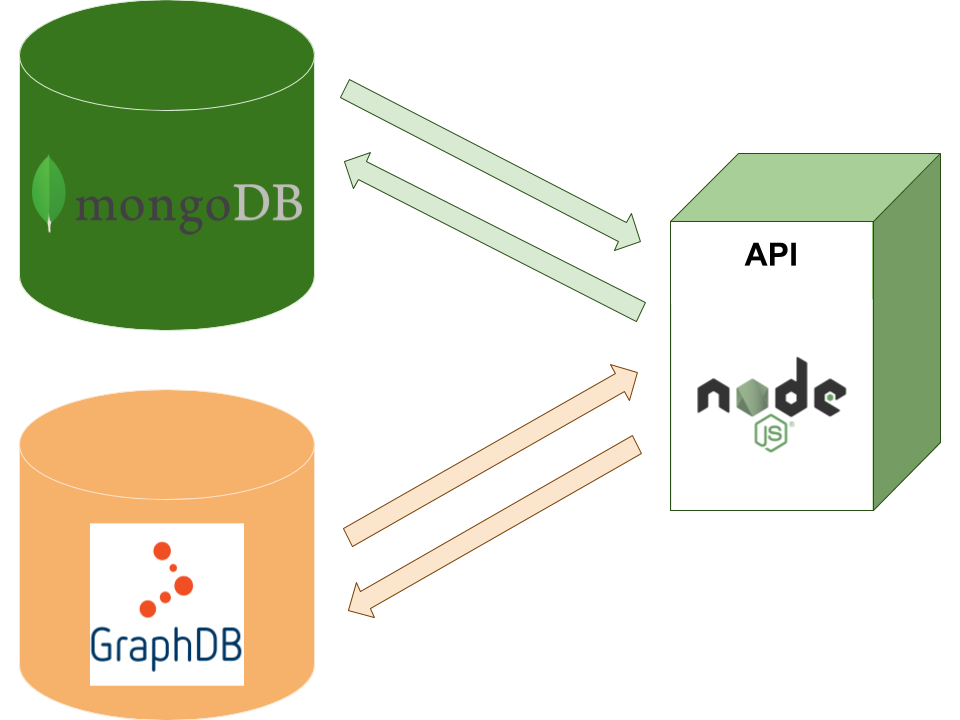
\includegraphics[width=10cm]{Pictures/backend.png}
    \caption{Estrutura do backend}
    \label{backend}
\end{figure}

Esta estrutura, demonstrada na figura acima (fig. \ref{backend}), é modular, ou seja, cada um dos três componentes identificados pode estar num servidor/máquina/\textit{container} diferente, o que permite escalar a API.

Nas próximas secções será aprofundado os vários constituintes e camadas da API.

\subsection{Modelos}

Nos \texttt{Models} define-se os \textit{schemas} das coleções de documentos da base de dados \textit{MongoDB}. Cada ficheiro \texttt{.js} corresponde a uma coleção, sendo que cada \texttt{schema} permite definir a estrutura de cada tipo de documento. Foram definidos os seguintes \textit{Schemas}/Documentos:

\paragraph{\textbf{User:}} representa um utilizador
    \begin{itemize}
        \item \texttt{name:} String obrigatória referente ao nome do utilizador;
        \item \texttt{email:} String obrigatória, única, ou seja sem repetição na base de dados, portanto pode servir de identificação, representado o email do utilizador;
        \item \texttt{password:} String obrigatória encriptada referente à password do utilizador;
        \item \texttt{stats:} lista com as estatísticas do utilizador;
            \begin{itemize}
                \item \texttt{id:} id (String) do \textit{Recording} a que se associa os valores seguintes;
                \item \texttt{views:} número de visualizações do utilizador deste \textit{Recording};
                \item \texttt{rating:} classificação dado pelo utilizador a este \textit{Recording}.
            \end{itemize}
        \item \texttt{favs:} lista de identificadores dos \textit{Recordings} favoritos do utilizador
    \end{itemize}

\paragraph{\textbf{Stats:}} salvaguarda as estatísticas de antigos utilizadores (utilizadores que apagaram a sua conta)
    \begin{itemize}
        \item \texttt{id:} id (String) do \textit{Recording} a que se associa os valores seguintes;
        \item \texttt{views:} número de visualizações do \textit{Recording} salvaguardadas;
        \item \texttt{avgRating:} classificação média do \textit{Recording} salvaguardada;
        \item \texttt{nRating:} número de utilizadores que classificaram o \textit{Recording}.
    \end{itemize}

\subsection{Controladores}

Os \texttt{controllers} possuem várias funções que permitem manusear os documentos e os seus valores. As coleções de documentos são estruturados por \texttt{Schemas} recorrendo ao \texttt{Mongoose}, sendo nos \texttt{Controllers} onde se encontram definidos a criação, atualização, destruição, listagem e obtenção de estatísticas dos mesmos. Apresentasse de seguida os \textit{controllers} dos \textit{models} \textit{User} e \textit{Stats} (quando se refere música assuma o mesmo que \textit{Recording}):

\paragraph{\textbf{User:}}
    \begin{itemize}
        \item \texttt{findOne}: Dado um email obtém a informação do utilizador com esse email associado;
        \item \texttt{getUser}: Dado um id obtém a informação do utilizador com esse id associado;
        \item \texttt{isValidPassword}: Dadas duas passwords, compara-as, verificando se são iguais;
        \item \texttt{createUser}: Dada a informação de um utilizador, encripta a password, criando, por fim, o utilizador;
        \item \texttt{updateUser}: Dada a informação a atualizar (\textit{name} e/ou \textit{email}) e o id do utilizador, atualiza a informação deste; esta função restringe o acesso, ou seja, apenas o próprio utilizador pode atualizar a sua informação;
        \item \texttt{updatePassword}: dado o id de um utilizador, a password atual e a nova password, verifica se a password atual está correta (se é igual à presente na base de dados), e em caso afirmativo, encripta a nova password e passa a ser a password atual do utilizador;
        \item \texttt{deleteUser}: dado um id de um utilizador, apaga-o;
        \item \texttt{getRecordingsUser}: dado um id de um utilizador, obtém uma lista com todas as estatisticas do utilizador (visualizações e classificações);
        \item \texttt{getMostRecordingsViewsUser}: dado um id de um utilizador, obtém uma lista das 10 músicas mais ouvidas/vistas pelo utilizador; cada elemento desta lista tem o id da música e o número de visualizações desta;
        \item \texttt{getMostRecordingsRatingUser}: dado um id de um utilizador, obtém uma lista das 10 músicas com maior classificação dada pelo utilizador; cada elemento desta lista tem o id da música e a classificação atribuída;
        \item \texttt{getRecordingUserRating}: dado um id de um utilizador e um id de uma música, devolve a classificação dada pelo utilizado à música; caso o utilizador não a tenha classificado, devolve 0;
        \item \texttt{updateViews}: dado um id de um utilizador e o id de uma música, soma mais uma visualização a essa música, caso as estatísticas para essa música já existam; caso não existam cria uma, com número de visualizações igual a 1 e classificação igual a 0;
        \item \texttt{updateRating}: dado um id de um utilizador, o id de uma música e a classificação a atribuir, caso as estatítiscas para esta música ja existam, atribui a nova classificação; caso não existam cria uma nova estatística para a música, com o número de visualizações igual a 0 e a classificação igual à que foi inserida.
        \item \texttt{getFavs}: dado um id de um utilizador, obtém a lista de favoritos do utilizador
        \item \texttt{addFav}: dado um id de um utilizador e o id da música, adiciona a música à lista de favoritos do utilizador
        \item \texttt{removeFav}: dado um id de um utilizador e o id da música, remove a música da lista de favoritos do utilizador
        \item \texttt{isFav}: dado um id de um utilizador e o id da música, verifica se a música está na lista de favoritos do utilizador

    \end{itemize}

\paragraph{\textbf{Stats:}}
    \begin{itemize}
        \item \texttt{createOrUpdate}: dado estatísticas de uma música (id, \textit{views}, \textit{rating}), agrega estes valores com os existentes, caso já exista o documento para o id desta música; caso ainda não exista é criado um;
        \item \texttt{getStats}: obtém todas as estatísticas, estejam elas presentes nos documentos \textit{Stats} ou nos utilizadores, agregando as estatísticas pelos ids das músicas;
        \item \texttt{getMostRecordingsViews}: obtém as 10 músicas mais ouvidas;
        \item \texttt{getMostRecordingsRating}: obtém as 10 músicas com maior classificação;
        \item \texttt{getRecordingStats}: dado o id de uma música, obtém as estatísticas para esta música;
        \item Nota: Para obter as estatísticas, foi necessário, como já referido, aceder aos documentos dos utilizadores a partir deste \texttt{controller}.
    \end{itemize}

Por outro lado, também é aqui nos \texttt{controllers} que são realizadas as \textit{queries} à base de dados \textit{GraphDB}. Por forma, a modularizar o código, no ficheiro \textit{execQuery.js} é definida a função \texttt{execQuery}, onde apenas recebe a \textit{query} a ser realizada, e devolve o resultado já ``limpo'', ou seja, uma lista de resultados, onde cada elemento, tem como atributos as variáveis devolvidas pela \textit{query} e como valor o seu valor obtido. A função \texttt{execQuery} já inclui o prefixo da ontologia pelo que na \textit{query} não é necessário indicar a totalidade do \textit{URI} bastando apenas colocar ``:'' quando se refere a um \textit{URI} da ontologia definida neste trabalho (ver \ref{ontologia}). Contudo, antes de fazer qualquer pedido com esta função é necessário definir o \texttt{hostname:porta} através da função \texttt{set} (basta apenas definir uma vez). Esta função (\texttt{set}) foi criada por forma a facilitar o \textit{deployment} do servidor bem como do \textit{GraphDB}. Todas as \textit{queries} realizadas são de leitura de informação, sendo estas dividas em ficheiros pela classe que questionam. Sendo assim, existem os seguintes \texttt{controllers} que questionam o \textit{GraphDB} de forma a obter informação de indivíduos da classe:

\paragraph{\textbf{Album:}}
    \begin{itemize}
        \item \texttt{listAlbums}: dado um \textit{offset}, lista os 50 albums (id e título do album) a partir do \textit{offset} da lista (ordenada (pelos títulos), foi removido ordenação por questões de performance) de todos os albums;
        \item \texttt{listAlbumsByFilter}: dado um \textit{offset} e um filtro, devolve o mesmo que o anterior contudo em vez da lista (ordenada, foi removido ordenação por questões de performance) ser de todos os albums, é apenas dos albums que começam pelo valor presente no filtro;
        \item \texttt{getAlbum}: dado o id de um album, obtém o título, e caso exista, data da primeira \textit{release}, sobre (\textit{about}) e desambiguação;
        \item \texttt{getURLs}: dado o id de um album, obtém os \textit{URLs} sobre o album, devolvendo uma lista onde cada elemento possui o nome do website e o \textit{URL};
        \item \texttt{getTracks}: dado o id de um album, obtém as músicas pertencentes ao album, devolvendo uma lista, em que cada elemento tem o id, título, duração e, caso exista, desambiguação de uma música;
        \item \texttt{getTags}: dado o id de um album, obtém as tags do album, através das tags pertencentes às músicas pertencentes ao album;
        \item \texttt{getArtistsCredit}: dado o id de um album, obtém os artistas do album através dos artistas associados às músicas pertencentes ao album.
    \end{itemize}

\paragraph{\textbf{Area:}}
    \begin{itemize}
        \item \texttt{listAreas}: dado um \textit{offset}, lista as 50 areas (id e nome da area) a partir do \textit{offset} da lista (ordenada (pelos nomes), foi removido ordenação por questões de performance) de todas os areas;
        \item \texttt{listAreasByFilter}: dado um \textit{offset} e um filtro, devolve o mesmo que o anterior contudo em vez da lista (ordenada, foi removido ordenação por questões de performance) ser de todas as areas, é apenas das areas que começam pelo valor presente no filtro;
        \item \texttt{getArea}: dado o id de uma area, obtém o nome, o tipo, e caso exista, sobre (\textit{about}) e desambiguação;
        \item \texttt{getAliases}: dado o id de uma area obtém os nomes alternativos para a area;
        \item \texttt{getPartOf}: dado o id de uma area obtém o id, nome e tipo das areas a que pertence;
        \item \texttt{getParts}: dado o id de uma area obtém o id, nome e tipo das areas que contém;
        \item \texttt{getURLs}: dado o id de uma area, obtém os \textit{URLs} sobre a area, devolvendo uma lista onde cada elemento possui o nome do website e o \textit{URL};
        \item \texttt{getArtists}: dado o id de uma area, obtém os artistas que são dessa area, devolvendo para cada artista o seu id e nome.
        \item \texttt{countriesWithMostArtists}: obtém uma lista de todos os paises, ordenados do país com mais artistas para o país com menos
        \item \texttt{countriesWithMostRecordings}: obtém uma lista de todos os paises, ordenados do país com mais músicas para o país com menos
        \item \texttt{countriesWithMostAlbums}: obtém uma lista de todos os paises, ordenados do país com mais albums para o país com menos
    \end{itemize}

\paragraph{\textbf{Artist:}}
    \begin{itemize}
        \item \texttt{listArtists}: dado um \textit{offset}, lista os 50 artistas (id e nome do artista) a partir do \textit{offset} da lista (ordenada (pelos nomes), foi removido ordenação por questões de performance) de todas os artistas;
        \item \texttt{listArtistsByFilter}: dado um \textit{offset} e um filtro, devolve o mesmo que o anterior contudo em vez da lista (ordenada, foi removido ordenação por questões de performance) ser de todos os artistas, é apenas dos artistas que começam pelo valor presente no filtro;
        \item \texttt{getArtist}: dado o id de um artista, obtém o nome, e caso exista, o tipo, o nome para ordenar, a data de nascimento/início, a data de falecimento/fim, o sexo, o id da area, o nome da area, sobre (\textit{about}) e desambiguação;
        \item \texttt{getAliases}: dado o id de um artista obtém os nomes alternativos para o artista;
        \item \texttt{getURLs}: dado o id de um artista, obtém os \textit{URLs} sobre o artista, devolvendo uma lista onde cada elemento possui o nome do website e o \textit{URL};
        \item \texttt{getRecordings}: dado o id de um artista, devolve o id e o título das músicas no qual o artista fez parte;
        \item \texttt{getTags}: dado o id de um artista, obtém as tags do artista, através das tags pertencentes às músicas no qual o artista fez parte;
        \item \texttt{getAlbums}: dado o id de um artista, obtém os albums do artista, ou seja, onde o artista possui músicas nas quais fez parte.
    \end{itemize}

\paragraph{\textbf{Recording:}}
    \begin{itemize}
        \item \texttt{listRecordings}: dado um \textit{offset}, lista as 50 músicas (id e título da música) a partir do \textit{offset} da lista (ordenada (pelos títulos), foi removido ordenação por questões de performance) de todas as músicas;
        \item \texttt{listRecordingsByFilter}: dado um \textit{offset} e um filtro, devolve o mesmo que o anterior contudo em vez da lista (ordenada, foi removido ordenação por questões de performance) ser de todas as músicas, é apenas das músicas que começam pelo valor presente no filtro;
        \item \texttt{getRecording}: dado o id de uma música, obtém o título, e caso exista, a duração, sobre (\textit{about}) e desambiguação;
        \item \texttt{getLanguages}: dado o id de uma música obtém as línguas usadas na música;
        \item \texttt{getTags}: dado o id de uma música, obtém as tags da música;
        \item \texttt{getURLs}: dado o id de uma música, obtém os \textit{URLs} sobre a música, devolvendo uma lista onde cada elemento possui o nome do website e o \textit{URL};
        \item \texttt{getArtistsCredit}: dado o id de uma música, devolve o id e o nome dos artistas que fizeram parte da música;
        \item \texttt{getAlbums}: dado o id de uma música, devolve os albums no qual a música faz parte;
        \item \texttt{searchForRecordings}: dados dois filtros, um para o nome de um artista e outro para um título de uma música, obtém o id, nome do artista e título de músicas em que o nome do artista comece pelo seu filtro e o título da música comece também pelo seu filtro.
    \end{itemize}

\subsection{Rotas}

As rotas encaminham os pedidos dos clientes de forma a realizarem a correta chamada de funções presentes nos \texttt{Controllers}, sendo que a rota para onde o utilizador é encaminhado varia consoante o \texttt{URL} e o método do pedido.
De seguida, apresentam-se as rotas, a função que é chamada para cada rota e é referido alguns passos adicionais que são realizados em alguns casos.

\paragraph{\textit{Controller} User: rota \texttt{/users} concatenada com:}
    \begin{itemize}
        \item método \texttt{GET}
            \begin{itemize}
                \item \texttt{/isAuthenticated} - devolve ``Authenticated'' se o utilizador estiver autenticado, caso contrário devolve ``Unauthorized'', permite saber se um utilizador está autenticado
                \item \texttt{/:id/favs} - \texttt{getFavs(:id)} se o ``:id'' for igual ao id do utilizador que está autenticado, senão devolve uma mensagem de erro
                \item \texttt{/:id/isFav/:idMusic} - \texttt{isFav(:id,:idMusic)} se o ``:id'' for igual ao id do utilizador que está autenticado, senão devolve uma mensagem de erro
                \item \texttt{/:id/statsMostViews} - \texttt{getMostRecordingsViewsUser(:id)} se o ``:id'' for igual ao id do utilizador que está autenticado, senão devolve uma mensagem de erro
                \item \texttt{/:id/statsMostRating} - \texttt{getMostRecordingsRatingUser(:id)} se o ``:id'' for igual ao id do utilizador que está autenticado, senão devolve uma mensagem de erro
                \item \texttt{/:id/stats?idRec=idRecI} - \texttt{getRecordingUserRating(:id, idRecI)} se o ``:id'' for igual ao id do utilizador que está autenticado, senão devolve uma mensagem de erro
                \item \texttt{/:id/stats} - \texttt{getRecordingsUser(:id)} se o ``:id'' for igual ao id do utilizador que está autenticado, senão devolve uma mensagem de erro
                \item \texttt{/:id} - \texttt{getUser(:id)} se o ``:id'' for igual ao id do utilizador que está autenticado, senão devolve uma mensagem de erro
            \end{itemize}
        \item método \texttt{POST}
            \begin{itemize}
                \item \texttt{/login} - permite a autenticação de um utilizador, caso o utilizador exista e a password seja a correta, gerando um \textit{token} que é enviado ao cliente. Esta parte será vista mais à frente (ver \ref{auth}) 
                \item \texttt{/} - \texttt{createUser(body)}
            \end{itemize}
        \item método \texttt{PUT}
            \begin{itemize}
                \item \texttt{/views/:id} - \texttt{updateViews(:id, body.idMusic)} se o ``:id'' for igual ao id do utilizador que está autenticado, senão devolve uma mensagem de erro
                \item \texttt{/rating/:id} - \texttt{updateRating(:id, body.idMusic, body.rating)} se o ``:id'' for igual ao id do utilizador que está autenticado, senão devolve uma mensagem de erro
                \item \texttt{/updPass/:id} - \texttt{updatePassword(:id, body.prevPass, body.newPass)} se o ``:id'' for igual ao id do utilizador que está autenticado, senão devolve uma mensagem de erro
                \item \texttt{/addFav/:id} - \texttt{addFav(:id, body.idMusic)} se o ``:id'' for igual ao id do utilizador que está autenticado, senão devolve uma mensagem de erro
                \item \texttt{/removeFav/:id} - \texttt{removeFav(:id, body.idMusic, body.rating)} se o ``:id'' for igual ao id do utilizador que está autenticado, senão devolve uma mensagem de erro
                \item \texttt{/:id} - \texttt{updateUser(:id, body)} se o ``:id'' for igual ao id do utilizador que está autenticado, senão devolve uma mensagem de erro
            \end{itemize}
        \item método \texttt{DELETE}
            \begin{itemize}
                \item \texttt{/:id} - \texttt{deleteUser(:id)} e para cada sub documento de estatísticas do utilizador apagado (\texttt{stat}) é a chamada a função \texttt{createOrUpdate(stat)} do \texttt{controller} Stats, se o ``:id'' for igual ao id do utilizador que está autenticado, senão devolve uma mensagem de erro
            \end{itemize}
    \end{itemize}

\paragraph{\textit{Controller} Stats: rota \texttt{/stats} concatenada com:}
    \begin{itemize}
        \item método \texttt{GET}
            \begin{itemize}
                \item \texttt{/mostViews} - \texttt{getMostRecordingsViews()} 
                \item \texttt{/mostRating} - \texttt{getMostRecordingsRating()} 
                \item \texttt{/:id} - \texttt{getRecordingStats(:id)} 
                \item \texttt{/} - \texttt{getStats()} 
            \end{itemize}
        \item método \texttt{POST}
            \begin{itemize}
                \item \texttt{/} - \texttt{createOrUpdate(body)}
            \end{itemize}
    \end{itemize}

\paragraph{\textit{Controller} Album: rota \texttt{/albums} concatenada com:}
    \begin{itemize}
        \item método \texttt{GET}
            \begin{itemize}
                \item \texttt{/:id/tags} - \texttt{getTags(:id)} 
                \item \texttt{/:id/tracks} - \texttt{getTracks(:id)} 
                \item \texttt{/:id/artistsCredit} - \texttt{getArtistsCredit(:id)} 
                \item \texttt{/:id/urls} - \texttt{getURLs(:id)} 
                \item \texttt{/:id} - \texttt{getAlbum(:id)} 
                \item \texttt{?offset=offsetI\&filter=filterI} - \texttt{listAlbumsByFilter(offsetI, filterI)}
                \item \texttt{?filter=filterI} - \texttt{listAlbumsByFilter(0, filterI)}
                \item \texttt{?offset=offsetI} - \texttt{listAlbums(offsetI)}
                \item \texttt{/} - \texttt{listAlbums(0)}
            \end{itemize}
    \end{itemize}

\paragraph{\textit{Controller} Area: rota \texttt{/areas} concatenada com:}
    \begin{itemize}
        \item método \texttt{GET}
            \begin{itemize}
                \item \texttt{/countriesWithMostAlbums?cache=true} - o mesmo que \texttt{countriesWithMostAlbums()} mas a partir da cache, visto que o resultado é estático
                \item \texttt{/countriesWithMostRecordings?cache=true} - o mesmo que \texttt{countriesWithMostRecordings()} mas a partir da cache, visto que o resultado é estático
                \item \texttt{/countriesWithMostArtists?cache=true} - o mesmo que \texttt{countriesWithMostArtists()} mas a partir da cache, visto que o resultado é estático
                \item \texttt{/countriesWithMostAlbums} - \texttt{countriesWithMostAlbums()}
                \item \texttt{/countriesWithMostRecordings} - \texttt{countriesWithMostRecordings()}
                \item \texttt{/countriesWithMostArtists} - \texttt{countriesWithMostArtists()}
                \item \texttt{/:id/aliases} - \texttt{getAliases(:id)}
                \item \texttt{/:id/artists} - \texttt{getArtists(:id)}
                \item \texttt{/:id/urls} - \texttt{getURLs(:id)}
                \item \texttt{/:id/parts} - \texttt{getParts(:id)}
                \item \texttt{/:id/partOf} - \texttt{getPartOf(:id)}
                \item \texttt{/:id} - \texttt{getArea(:id)}
                \item \texttt{?offset=offsetI\&filter=filterI} - \texttt{listAreasByFilter(offsetI, filterI)}
                \item \texttt{?filter=filterI} - \texttt{listAreasByFilter(0, filterI)}
                \item \texttt{?offset=offsetI} - \texttt{listAreas(offsetI)}
                \item \texttt{/} - \texttt{listAreas(0)}
            \end{itemize}
    \end{itemize}

\paragraph{\textit{Controller} Artist: rota \texttt{/artists} concatenada com:}
    \begin{itemize}
        \item método \texttt{GET}
            \begin{itemize}
                \item \texttt{/:id/tags} -  \texttt{getTags(:id)}
                \item \texttt{/:id/albums} - \texttt{getAlbums(:id)}
                \item \texttt{/:id/recordings} - \texttt{getRecordings(:id)}
                \item \texttt{/:id/urls} - \texttt{getURLs(:id)}
                \item \texttt{/:id/aliases} - \texttt{getAliases(:id)}
                \item \texttt{/:id} - \texttt{getArtist(:id)}
                \item \texttt{?offset=offsetI\&filter=filterI} - \texttt{listArtistsByFilter(offsetI, filterI)}
                \item \texttt{?filter=filterI} - \texttt{listArtistsByFilter(0, filterI)}
                \item \texttt{?offset=offsetI} - \texttt{listArtists(offsetI)}
                \item \texttt{/} - \texttt{listArtists(0)}
            \end{itemize}
    \end{itemize}

\paragraph{\textit{Controller} Recording: rota \texttt{/recordings} concatenada com:}
    \begin{itemize}
        \item método \texttt{GET}
            \begin{itemize}
                \item \texttt{/search?name=nameI\&title=titleI} - \texttt{searchForRecordings(nameI, titleI)}
                \item \texttt{/:id/albums} - \texttt{getAlbums(:id)}
                \item \texttt{/:id/artistsCredit} - \texttt{getArtistsCredit(:id)}
                \item \texttt{/:id/urls} - \texttt{getURLs(:id)}
                \item \texttt{/:id/languages} - \texttt{getLanguages(:id)}
                \item \texttt{/:id/tags} - \texttt{getTags(:id)}
                \item \texttt{/:id} - \texttt{getRecording(:id)}
                \item \texttt{?offset=offsetI\&filter=filterI} - \texttt{listRecordingsByFilter(offsetI, filterI)}
                \item \texttt{?filter=filterI} - \texttt{listRecordingsByFilter(0, filterI)}
                \item \texttt{?offset=offsetI} - \texttt{listRecordings(offsetI)}
                \item \texttt{/} - \texttt{listRecordings(0)}
            \end{itemize}
    \end{itemize}

\subsection{Autenticação} \label{auth}

As rotas da API estão quase todas protegidas à exceção de duas, \texttt{GET} de \texttt{/users/login} e \texttt{POST} de \texttt{/users}. A primeira rota não está protegida porque é onde os utilizadores podem realizar \textit{login}, e que em caso de autenticação com sucesso é gerado um \texttt{token} que é enviado para o utilizador. Já a segunda rota permite a criação (registo) de utilizadores.

De forma a aceder às rotas protegidas, os clientes tem de enviar o \texttt{token}, que lhes foi fornecido, nas \texttt{headers} do pedido, mais precisamente na \textit{header} \texttt{Authorization}, sendo o valor a colocar neste campo igual a \texttt{Bearer \$\{token\}}.

\begin{figure}[H]
    \centering
    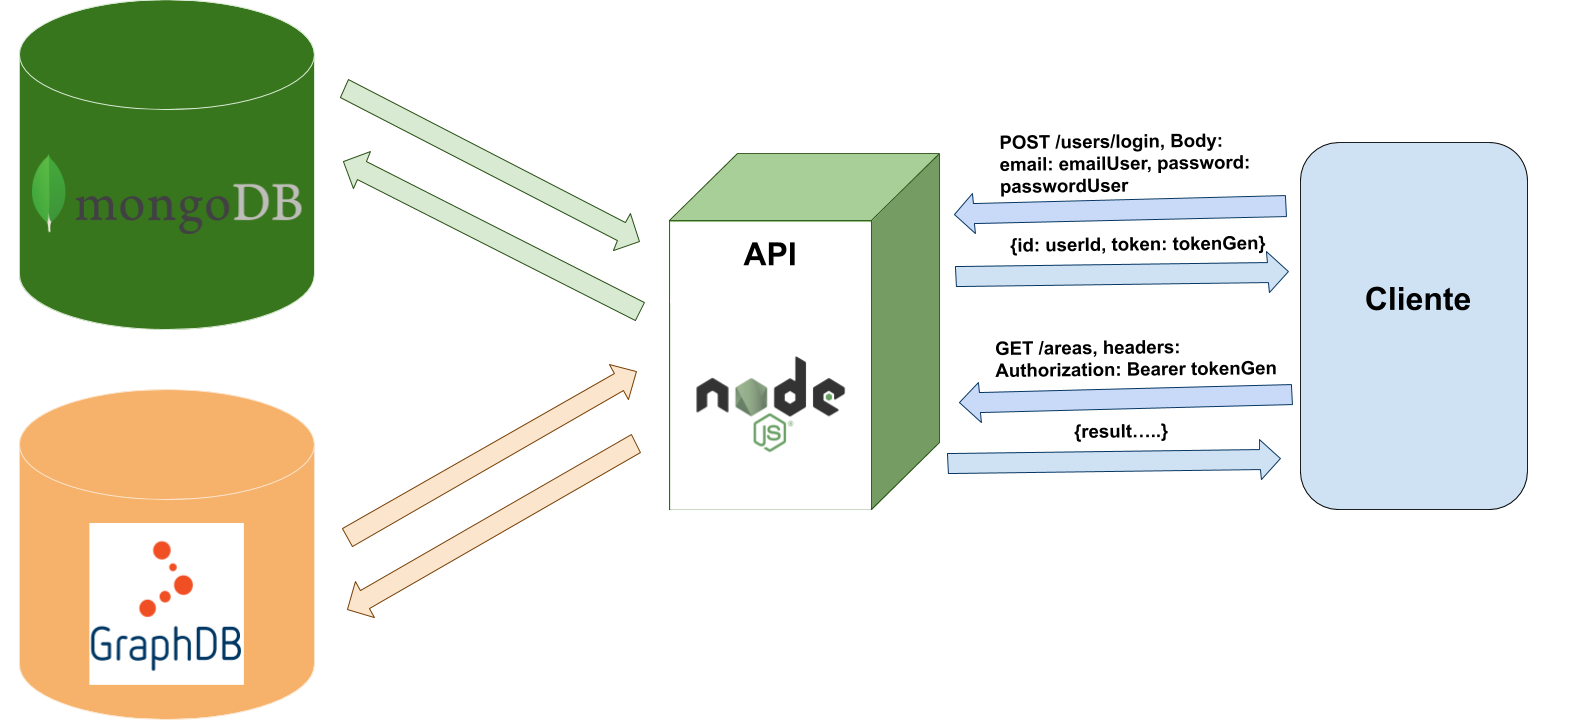
\includegraphics[width=15cm]{Pictures/exeAuth.png}
    \caption{Um exemplo de um login e posterior pedido com envio do \textit{token}}
    \label{exe_auth}
\end{figure}

O \textit{token} tem um tempo de validade, pelo que ao fim de 30 minutos expira, sendo necessária nova autenticação pelo utilizador.

A autenticação é realizada com a ajuda do \texttt{passport-local}. De forma a gerar o \textit{token} recorre-se ao \texttt{jsonwebtoken} usando uma chave privada para gerar o \textit{token} através do algoritmo RS256 (\textit{RSA Signature with SHA-256}). Já na verificação do \textit{token} é utilizado o \texttt{passport-jwt} com a tática de extração \texttt{fromAuthHeaderAsBearerToken}, daí a necessidade de colocar o \textit{token} nas headers dos pedidos como indicado. Esta verificação recorre à chave pública para confirmar a validade do \textit{token}. Por fim, é importante referir que no \textit{deployment} deste servidor é de extrema importancia, trocar a chave privada e a chave pública, visto este trabalho estar disponível publicamente.

\section{Interface}

A interface foi desenvolvida através da \textit{framework} \texttt{Vue.js} e a \textit{framework} de material \texttt{Vuetify.js} baseada no \textit{Material Design} da \textit{Google}. Esta interface estará no lado do utilizador, enquanto que a API está presente num servidor. Claro, contudo, esta interface tem de ser armazenada num servidor, de forma aos clientes/utilizadores fazerem o download desta interface, para posteriormente acederem diretamente à API através da interface.

Quanto a imagens usadas na interface, estas estão armazenadas em \texttt{public/static/}.

\begin{figure}[H]
    \centering
    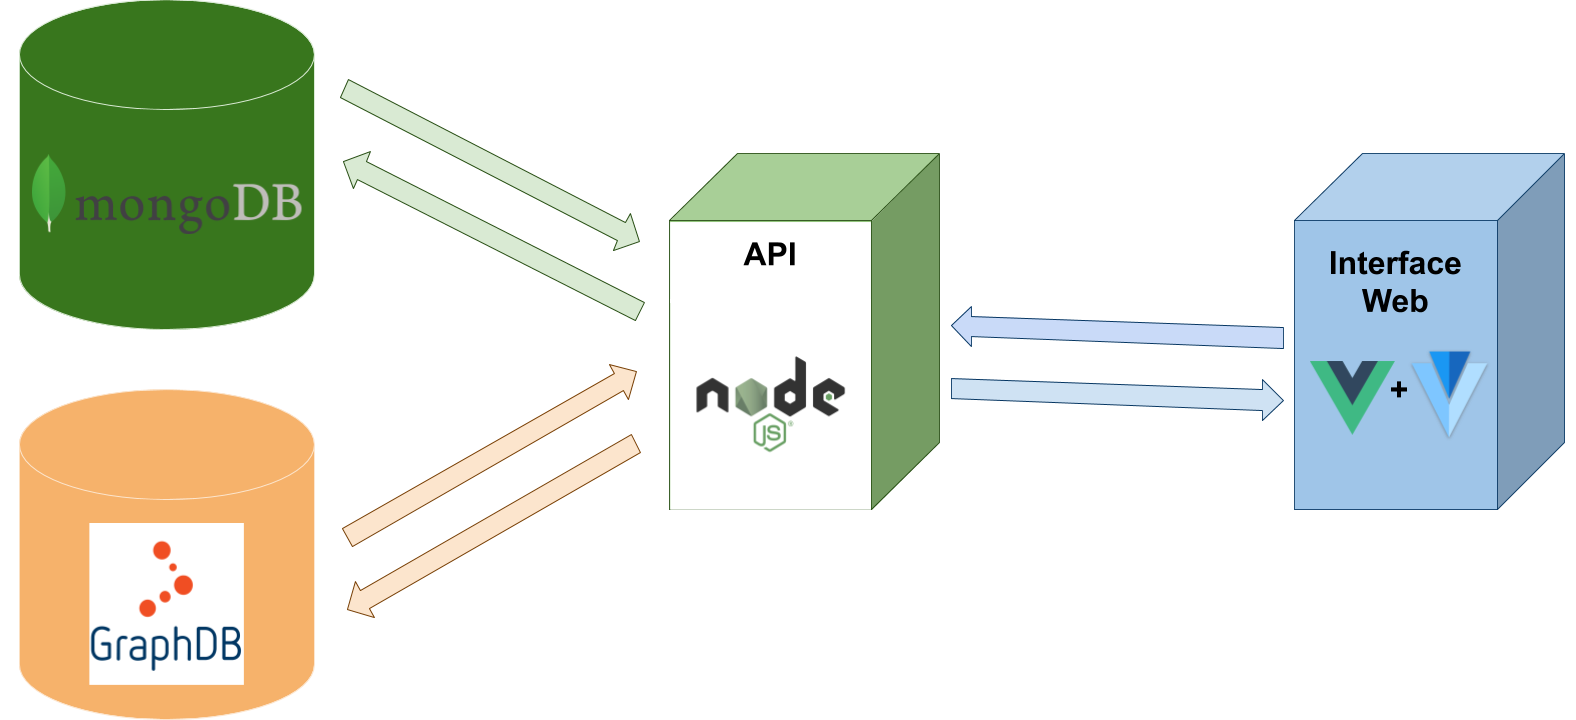
\includegraphics[width=12cm]{Pictures/backend_frontend.png}
    \caption{Estrutura do backend e frontend}
    \label{backend_frontend}
\end{figure}

Já em relação ao aspeto visual da interface, ela possui um \textit{footer}, que aparece em todas as páginas, e como tal, foi definida na \texttt{App.vue}. Este \textit{footer} possui allguns \textit{URLs} importantes, desde API usadas, ao \textit{URL} onde se pode verificar o código produzido.

Já na \texttt{main.js} é definida uma variável global (\texttt{\$urlAPI}) onde está presente o \textit{URL} da API, de forma a tornar o código mais limpo. O valor desta variável toma o valor da variável ambiente \texttt{VUE\_APP\_SERVER\_URL} definida em \texttt{.env} por forma a uma maior facilidade de \textit{deployment} da interface. É também aqui importado uma \textit{package} \textit{wrapper} da API do \textit{iframe} do \textit{Youtube}.

De seguida, serão apresentadas as várias camadas da interface.

\subsection{Rotas}

Visto que foi usada um versão do \textit{Vue.js} com um \textit{router} existem rotas a definir, indicando para que vista as mesmas redirecionam. Apresenta-se, de seguida, as rotas definidas (presentes no ficheiro \textit{router.js}):

\begin{itemize}
    \item Rota \texttt{/recordingsSearch} $\to$ vista \texttt{RecordingsSearch.vue}
    \item Rota \texttt{/recordings/:id} $\to$ vista \texttt{Recording.vue}
    \item Rota \texttt{/areas/:id} $\to$ vista \texttt{Area.vue}
    \item Rota \texttt{/artists/:id} $\to$ vista \texttt{Artist.vue}
    \item Rota \texttt{/albums/:id} $\to$ vista \texttt{Album.vue}
    \item Rota \texttt{/userSettings/:id} $\to$ vista \texttt{UserSettings.vue}
    \item Rota \texttt{/recordings} $\to$ vista \texttt{Recordings.vue}
    \item Rota \texttt{/areas} $\to$ vista \texttt{Areas.vue}
    \item Rota \texttt{/artists} $\to$ vista \texttt{Artists.vue}
    \item Rota \texttt{/albums} $\to$ vista \texttt{Albums.vue}
    \item Rota \texttt{/favs} $\to$ vista \texttt{Favs.vue}
    \item Rota \texttt{/index} $\to$ vista \texttt{Index.vue}
    \item Rota \texttt{/signup} $\to$ vista \texttt{SignUp.vue}
    \item Rota \texttt{/} $\to$ vista \texttt{Login.vue}
\end{itemize}

\subsection{Vistas}

As vistas definidas são bastante parecidas umas com as outras, tendo apenas algumas pequenas diferenças. 

Todas as vistas importam o componente com o mesmo nome que a vista, ou seja, por exemplo a vista \texttt{Areas.vue} importa o componente \texttt{Areas.vue}.

As vistas \texttt{Index.vue}, \texttt{Recordings.vue}, \texttt{Areas.vue}, \texttt{Artists.vue}, \texttt{Albums.vue}, \texttt{RecordingsSearch.vue}, \texttt{Recording.vue}, \texttt{Area.vue}, \texttt{Artist.vue}, \texttt{Album.vue}, \texttt{UserSettings.vue} e \texttt{Favs.vue} verificam se o utilizador está autenticado, em caso afirmativo é feito a renderização da página; em caso negativo o utilizador é redirecionado para a página de \textit{login} (rota \texttt{/}).

Em adição, as vistas \texttt{Recording.vue}, \texttt{Area.vue}, \texttt{Artist.vue} e \texttt{Album.vue}, passam um argumento para o componente. Este argumento é o id do individuo (\textit{Recording}, \textit{Area}, \textit{Artist} ou \textit{Album} respetivamente). A vista \texttt{UserSettings.vue} também passa um argumento para o componente, contudo este argumento é o id do utilizador.

Por fim, as vistas \texttt{Login.vue} e \texttt{SignUp.vue} verificam se o utilizador está autenticado, em caso afirmativo, o utilizador é redirecionado para a página inicial (vista \texttt{Index.vue}, rota \texttt{/index}); em caso negativo a página é renderizada.

\subsection{Componentes}

Os componentes permitem a modularização das páginas web, fomentando uma melhor codificação.

Visto existirem várias funções que são usadas em vários componentes, foram criados os seguintes ficheiros:

\paragraph{\texttt{auth.js}:}\mbox{}\\

Possui duas funções, \texttt{isAuthenticated} e \texttt{logout}. A primeira, pergunta à API se o utilizador está autenticado, caso não esteja, apaga da \textit{local storage} o \textit{token} e o id do utilizador. Já o \texttt{logout} apaga da \textit{local storage} o \textit{token} e o id do utilizador, sem verificar se ainda está autenticado. Ou seja, como foi dado a entender, durante a sessão de um utilizador, é guardado o seu id bem como o seu \textit{token} na \textit{local storage}.

\paragraph{\texttt{request.js}:}\mbox{}\\

Este ficheiro foi criado de forma a possuir funções que simplifiquem o uso da \textit{package} \texttt{axios}, ou seja, a realização de pedidos \textit{web} com a colocação em cabeçalho do \textit{token} do utilizador. Neste ficheiro está presente três funções, \textit{getAPI}, \textit{putAPI} e \textit{deleteAPI}. A função \textit{getAPI} recebe como argumento um \textit{url} para onde é feito um pedido \texttt{GET}. Já a função \textit{putAPI} para além de um \textit{url}, recebe também dados a enviar como argumento, realizando um pedido \texttt{PUT} desses dados para o \textit{url} fornecido. Por fim, o \textit{deleteAPI} recebe como argumento um \textit{url} para onde é feito um pedido \texttt{DELETE}. Como já referido estas três funções colocam nas \textit{headers} o \textit{token} do utilizador da forma já descrita na secção \ref{auth}.

\vspace{10px}

Antes de apresentar os componentes é importante referir que os componentes \texttt{Album.vue}, \texttt{Area.vue}, \texttt{Artist.vue} e \texttt{Recording.vue}, que apresentam um campo chamado \textit{about}, realizam o processamento deste campo, visto o mesmo possuir uma sintaxe própria, passível de ser representada em \texttt{HTML}.~\cite{mbAnnotation}. Esta sintaxe, foi convertida da seguinte forma:
\begin{itemize}
    \item \texttt{''pal''} (itálico) $\to$ \verb|<i>pal</i>|
    \item \texttt{'''pal'''} (bold) $\to$ \verb|<b>pal</b>|
    \item \texttt{----} (linha horizontal) $\to$ \verb|<hr>|
    \item \texttt{=title=} (título 1) $\to$ \verb|<h4>title</h4>|
    \item \texttt{==title==} (título 2) $\to$ \verb|<h5>title</h5>|
    \item \texttt{===title===} (título 3) $\to$ \verb|<h6>title</h6>|
    \item \texttt{[url]} (url) $\to$ \verb|<a href=url>url</a>|
    \item \texttt{[url|desc]} (url) $\to$ \verb|<a href=url>desc</a>|
\end{itemize}

De seguida apresentam-se os componentes criados.

\paragraph{\texttt{Login.vue}:}\mbox{}\\

Página onde se realiza o login, possui um formulário para preencher o email e a password. Possui ainda dois botões, um para autenticar e outro para ser redirecionado para a página de registo.

\paragraph{\texttt{SignUp.vue}:}\mbox{}\\

Página onde os utilizadores podem se registar. Possui um formulário, onde o utilizador necessita de indicar nome, email, password, repetir a password e depois de tudo ser validado (de forma a validar foi usado \href{https://vuelidate.netlify.com/}{\texttt{vuelidate}}) o botão para submeter o registo fica disponível. Quando o utilizador carregar para se registar, é redirecionado para a página de login, sendo mostrado uma mensagem de sucesso se o registo for efetuado com sucesso, ou pelo contrário se não tiver sucesso, aparece uma mensagem de erro. Possui também um botão \textit{Back to Login}, para voltar à página de login.

\paragraph{\texttt{Toolbar.vue}:}\mbox{}\\

Componente usado por quase todos os componentes, com a exceção dos componentes \texttt{Login.vue} e \texttt{SignUp.vue}. Este componente representa a barra de ferramentas superior que se encontra em grande parte das páginas. Nesta barra está presente vários links para diferentes páginas da interface, o primeiro onde está o nome da aplicação e o seu símbolo, redireciona para a página inicial (\texttt{/index}). Depois por ordem, links para \textit{Recordings} favoritos do utilizador, listagem de \textit{Albums}, \textit{Recordings}, \textit{Artists} e \textit{Areas}, para a página de configuração do utilizador e por fim \textit{Logout}. Quando o utilizador está numa destas páginas, a barra de ferramentas sinaliza a mesma ao usar uma cor diferente para o botão associada a essa página.

Para além disso, esta barra, por vezes, apresenta uma caixa de texto por forma a filtrar os resultados disponíveis ou para pesquisar. Quando se está nas páginas de listagem de \textit{Albums}, \textit{Recordings}, \textit{Artists} e \textit{Areas} esta caixa de texto permite filtrar os resultados. Nas restantes páginas em que aparece (página de um individuo \textit{Album}, \textit{Recording}, \textit{Artist} ou \textit{Area}, na página inicial \textit{Index} e na página de favoritos do utilizador \textit{Favs}), esta caixa de texto permite pesquisar por artista mais música com o formato ``\textit{Artist}-\textit{Recording}''.

\paragraph{\texttt{Index.vue}:}\mbox{}\\

Página inicial da interface. Apresenta estatísticas do utilizador e da aplicação, como as músicas mais ouvidas e com melhor classificação, entre outras (ver \ref{tema}). Ao carregar numa das músicas, albums, artistas ou areas, o utilizador é redirecionado para a página desse individuo.

\paragraph{\texttt{Albums.vue}:}\mbox{}\\

Lista todos os albums, mas por partes de 50 albums, devido à grande quantidade de albums. Ao fim dos 50 albums, apresenta-se um botão, de forma a obter os próximos 50 albums. Todos os albums renderizados, são clicáveis de forma a obter mais informação (redirecionamento para a página do album).

\paragraph{\texttt{Areas.vue}:}\mbox{}\\

Lista todos os areas, mas por partes de 50 areas, devido à grande quantidade de areas. Ao fim das 50 areas, apresenta-se um botão, de forma a obter as próximas 50 areas. Todas as areas renderizadas, são clicáveis de forma a obter mais informação (redirecionamento para a página da area).

\paragraph{\texttt{Artists.vue}:}\mbox{}\\

Lista todos os artistas, mas por partes de 50 artistas, devido à grande quantidade de artistas. Ao fim dos 50 artistas, apresenta-se um botão, de forma a obter os próximos 50 artistas. Todos os artistas renderizados, são clicáveis de forma a obter mais informação (redirecionamento para a página do artista).

\paragraph{\texttt{Recordings.vue}:}\mbox{}\\

Lista todos as músicas, mas por partes de 50 músicas, devido à grande quantidade de músicas. Ao fim das 50 músicas, apresenta-se um botão, de forma a obter as próximas 50 músicas. Todas as músicas renderizadas, são clicáveis de forma a obter mais informação (redirecionamento para a página da música).

\paragraph{\texttt{RecordingsSearch.vue}:}\mbox{}\\

Página para onde o utilizador é redirecionado quando pesquisa na caixa de texto com o formato ``\textit{Artist}-\textit{Recording}''. Lista as músicas que obedecem à pesquisa, sendo possível obter mais informação da música ao clicar nela (o utilizador é redirecionado para a página da música).

\paragraph{\texttt{Album.vue}:}\mbox{}\\

Página que apresenta toda a informação de um determinado individuo da classe \textit{Album}. Apresenta também a classificação e o rating do album. (ver \ref{tema})

\paragraph{\texttt{Area.vue}:}\mbox{}\\

Página que apresenta toda a informação de um determinado individuo da classe \textit{Area}. (ver \ref{tema})

\paragraph{\texttt{Artist.vue}:}\mbox{}\\

Página que apresenta toda a informação de um determinado individuo da classe \textit{Artist}. Apresenta também a classificação e o rating do artista, bem como as 10 músicas mais ouvidas e mais bem classificadas do artista. (ver \ref{tema})

\paragraph{\texttt{Recording.vue}:}\mbox{}\\

Página que apresenta toda a informação de um determinado individuo da classe \textit{Recording}. Apresenta também a classificação e o rating da música. Para além disso mostra o vídeo da música (quando possível, nem sempre apresenta o vídeo correto) e as \textit{lyrics} da música. As \textit{lyrics} da música são obtidas a partir de duas APIs diferentes, \textit{musixmatch} e \textit{Chartlyrics}. A primeira API, apenas apresenta 30\% da música, visto estar a ser utilizado uma versão gratuita. Futuramente é necessário alterar o \textit{token} usado para aceder a esta API (\textit{musixmatch}) seja por questões de segurança ou para usar uma versão paga que apresenta toda a letra da música. Por fim, apresenta também um botão por forma ao utilizador adicionar/remover a música aos/dos favoritos.

\paragraph{\texttt{UserSettings.vue}:}\mbox{}\\

Nesta página, estão presentes dois formulários onde o utilizador pode, num deles atualizar a sua password e no outro atualizar a sua informação (nome e email). Os campos são igualmente verificados com \texttt{vuelidate}.

\paragraph{\texttt{Favs.vue}:}\mbox{}\\

Página que apresenta a listagem de todas as músicas favoritas do utilizador. É possível, através de dois botões, remover uma música dos favoritos ou aceder à página da música.

\paragraph{\texttt{Youtube.vue}:}\mbox{}\\

Componente usado pela página onde se apresenta um individuo da classe \textit{Recording}. Permite pesquisar vídeos do \textit{YouTube} por uma \textit{string} e mostrar o vídeo que possui o título que mais se assemelha a essa \textit{string}.

\section{Instalação}

Antes de explicar a instalação, é importante referir que ao correr o servidor API, o mesmo, aceita dois parametros, \texttt{hostname + porta} do MongoDB e do GraphDB. Permite que na altura de instalação se possa agilizar mais facilmente o escalonamento da aplicação. Também nesse sentido, na interface existe um ficheiro \texttt{.env}, que possui a variável de ambiente \texttt{VUE\_APP\_SERVER\_URL}, por forma a indicar à interface qual é o \texttt{hostname + porta} do servidor API.

Todo o código produzido pode ser descarregado a partir do repositório disponível no \texttt{GitHub} em \url{https://github.com/jcm300/Musike}. 

Em relação à instalação propriamente dita, pode ser realizada de várias formas, seja criando a ontologia de raíz (envolvendo conversão do dataset JSON) com posterior instalação da aplicação; seja usar a ontologia já criada com posterior instalação da aplicação; ou, por fim, através da utilização de containers (\textit{Docker}).

\subsection{Instalação com criação da ontologia com posterior instalação da aplicação}

Podemos dividir esta fase em duas partes, criação da ontologia e instalação da aplicação.

\paragraph{Criação da ontologia:}\mbox{}\\

Tem como dependências \texttt{git} e \texttt{Node.js}.

\begin{framed}
\begin{minted}{bash}
# clonar repositório por ssh
git clone git@github.com:jcm300/Musike.git
# ou por https
git clone https://github.com/jcm300/Musike.git

# entrar no diretório
cd Musike

# descomprimir dataset em JSON
cd datasets/JSON
cat artist_aa artist_ab artist_ac artist_ad artist_ae artist_af artist_ag \ 
    artist_ah artist_ai > artist.tar.xz
cat release-group_aa release-group_ab release-group_ac > release-group.tar.xz
cat release_aa release_ab release_ac release_ad release_ae release_af release_ag \ 
    release_ah release_ai release_aj release_ak release_al release_am release_an \
    release_ao release_ap release_aq release_ar release_as release_at release_au \
    release_av release_aw release_ax release_ay release_az release_ba release_bb \
    release_bc release_bd release_be release_bf release_bg release_bh release_bi \
    release_bj release_bk release_bl release_bm release_bn release_bo release_bp \
    release_bq release_br release_bs release_bt release_bu release_bv release_bw \
    release_bx release_by release_bz release_ca release_cb release_cc release_cd \
    release_ce release_cf release_cg release_ch release_ci release_cj release_ck \
    release_cl release_cm release-group_aa release-group_ab \
    release-group_ac > release.tar.xz
cat work_aa work_ab work_ac work_ad > work.tar.xz
tar xf area.tar.xz
tar xf artist.tar.xz
tar xf recording.tar.xz
tar xf release.tar.xz #CUIDADO: este ocupa 230gb
tar xf release-group.tar.xz
tar xf work.tar.xz

# preparar ficheiros para converter
mv mbdump/area area.json
mv mbdump/artist artist.json
mv mbdump/recording recording.json
mv mbdump/release release.json
mv mbdump/release-group release-group.json
mv mbdump/work work.json

# converter ficheiros json, criando finalmente a ontologia
cd ../../jsonTOturtle
./convert.sh

# a ontologia criada estará em:
cd ../datasets/Turtle
# com o nome igual a MusicBrainz.ttl 
\end{minted}
\end{framed}

\paragraph{Instalação da aplicação:}\mbox{}\\

Por forma a instalar a aplicação é necessário instalar, \texttt{Java 8} (dependência do \texttt{GraphDB}), \texttt{GraphDB}, \texttt{MongoDB} e \texttt{Node.js}.

\begin{framed}
\begin{minted}{bash}
# criar uma pasta graph-import na home do utilizador
mkdir ~/graph-import

# mover ontologia para a pasta
mv MusicBrainz.ttl ~/graph-import

# Correr GraphDB e no GraphDB Workbench criar um repositório com id igual 
# a "musicbrainz" e importar a ontologia para esse repositório

cd ../../src # mover para a pasta Musike/src

# alterar forma como é iniciado o GraphDB na script install.sh, caso seja necessário,
# visto que assume que o GraphDB está instalado em Musike/src/graphdb-free-8.9.0

# instalar dependências do node.js e iniciar GraphDB, MongoDB, servidor API e interface
./install.sh i

# depois de correr uma primeira vez o comando anterior, sempre que se pretender iniciar,
# ou seja, iniciar GraphDB, MongoDB, servidor API e interface basta correr
./install.sh r
\end{minted}
\end{framed}

\subsection{Instalação usando ontologia já criada com posterior instalação da aplicação}

Esta instalação também pode ser dividida em duas partes, importação da ontologia e instalação da aplicação.

\paragraph{Importação da ontologia:}\mbox{}\\

Em primeiro lugar, realiza-se a clonagem do repositório:

\begin{framed}
\begin{minted}{bash}
# clonar repositório por ssh
git clone git@github.com:jcm300/Musike.git
# ou por https
git clone https://github.com/jcm300/Musike.git

cd Musike
\end{minted}
\end{framed}

De seguida, instalasse \texttt{Java 8} (dependência do \texttt{GraphDB}).

O próximo passo pode ser realizado de duas formas, importação da ontologia ou usar o GraphDB incluido no repositório que já inclui a importação da ontologia. No primeiro método segue-se os passos iniciais da instalação anterior ou seja:

\begin{framed}
\begin{minted}{bash}
#Instalar GraphDB

# descomprimir ontologia já criada
cd datasets/Turtle
cat MusicBrainz.ttl.gz_aa MusicBrainz.ttl.gz_ab MusicBrainz.ttl.gz_ac \
    MusicBrainz.ttl.gz_ad MusicBrainz.ttl.gz_ae MusicBrainz.ttl.gz_af \
    MusicBrainz.ttl.gz_ag MusicBrainz.ttl.gz_ah MusicBrainz.ttl.gz_ai \
    MusicBrainz.ttl.gz_aj MusicBrainz.ttl.gz_ak MusicBrainz.ttl.gz_al \
    MusicBrainz.ttl.gz_am MusicBrainz.ttl.gz_an MusicBrainz.ttl.gz_ao \
    MusicBrainz.ttl.gz_ap MusicBrainz.ttl.gz_aq MusicBrainz.ttl.gz_ar \
    MusicBrainz.ttl.gz_as MusicBrainz.ttl.gz_at MusicBrainz.ttl.gz_au \
    MusicBrainz.ttl.gz_av MusicBrainz.ttl.gz_aw MusicBrainz.ttl.gz_ax \
    MusicBrainz.ttl.gz_ay MusicBrainz.ttl.gz_az MusicBrainz.ttl.gz_ba \
    MusicBrainz.ttl.gz_bb MusicBrainz.ttl.gz_bc MusicBrainz.ttl.gz_bd \
    MusicBrainz.ttl.gz_be MusicBrainz.ttl.gz_bf MusicBrainz.ttl.gz_bg \
    MusicBrainz.ttl.gz_bh MusicBrainz.ttl.gz_bi MusicBrainz.ttl.gz_bj \
    MusicBrainz.ttl.gz_bk MusicBrainz.ttl.gz_bl MusicBrainz.ttl.gz_bm \
    MusicBrainz.ttl.gz_bn > MusicBrainz.ttl.gz
gunzip -k MusicBrainz.ttl.gz

# criar uma pasta graph-import na home do utilizador
mkdir ~/graph-import

# mover ontologia para a pasta
mv MusicBrainz.ttl ~/graph-import

# Correr GraphDB e no GraphDB Workbench criar um repositório com id igual
# a "musicbrainz" e importar a ontologia para esse repositório

cd ../../src # mover para a pasta Musike/src

# alterar forma como é iniciado o GraphDB na script install.sh, caso seja necessário,
# visto que assume que o GraphDB está instalado em Musike/src/graphdb-free-8.9.0
\end{minted}
\end{framed}

O segundo método é usar o \texttt{GraphDB} incluido no repositório no qual, já inclui a ontologia importada bastando seguir os seguintes passos:

\begin{framed}
\begin{minted}{bash}
# descomprimir GraphDB
cd src/graphdb-free-8.9.0
cat graph.tar.gz_aa graph.tar.gz_ab graph.tar.gz_ac graph.tar.gz_ad graph.tar.gz_ae \
    graph.tar.gz_af graph.tar.gz_ag graph.tar.gz_ah graph.tar.gz_ai graph.tar.gz_aj \
    graph.tar.gz_ak graph.tar.gz_al graph.tar.gz_am graph.tar.gz_an graph.tar.gz_ao \
    graph.tar.gz_ap graph.tar.gz_aq graph.tar.gz_ar graph.tar.gz_as graph.tar.gz_at \
    graph.tar.gz_au graph.tar.gz_av graph.tar.gz_aw graph.tar.gz_ax graph.tar.gz_ay \
    graph.tar.gz_az graph.tar.gz_ba graph.tar.gz_bb graph.tar.gz_bc graph.tar.gz_bd \
    graph.tar.gz_be graph.tar.gz_bf graph.tar.gz_bg graph.tar.gz_bh graph.tar.gz_bi \
    graph.tar.gz_bj graph.tar.gz_bk graph.tar.gz_bl graph.tar.gz_bm graph.tar.gz_bn \
    graph.tar.gz_bo graph.tar.gz_bp graph.tar.gz_bq graph.tar.gz_br graph.tar.gz_bs \
    graph.tar.gz_bt graph.tar.gz_bu graph.tar.gz_bv graph.tar.gz_bw graph.tar.gz_bx \
    graph.tar.gz_by graph.tar.gz_bz graph.tar.gz_ca graph.tar.gz_cb graph.tar.gz_cc \
    graph.tar.gz_cd graph.tar.gz_ce graph.tar.gz_cf > graph.tar.gz
tar -xf graph.tar.gz

cd .. # mover para a pasta Musike/src
\end{minted}
\end{framed}

\paragraph{Instalação da aplicação:}\mbox{}\\

Por forma a instalar a aplicação é necessário instalar, \texttt{MongoDB} e \texttt{Node.js}.

\begin{framed}
\begin{minted}{bash}
# instalar dependências do node.js e iniciar GraphDB, MongoDB, servidor API e interface
./install.sh i

# depois de correr uma primeira vez o comando anterior, sempre que se pretender iniciar,
# ou seja, iniciar GraphDB, MongoDB, servidor API e interface basta correr
./install.sh r
\end{minted}
\end{framed}

\subsection{Instalação através de containers (\texttt{Docker})}

A instalação através de containers é a menos trabalhosa e mais simples contudo, normalmente possui pior performance em relação a uma instalação sobre um sistema operativo. Logo é deixado à escolha do utilizador/administrador o método que pretende usar para instalar.

Portanto, para instalar tudo através de \textit{containers}, o primeiro passo é instalar o \texttt{docker} e o \texttt{docker-compose}. De seguida, os passos a realizar são os seguintes:

\small
\begin{framed}
\begin{minted}{bash}
# obter o ficheiro docker-compose para proceder à criação dos containers
wget https://raw.githubusercontent.com/jcm300/Musike/master/src/docker-compose_without_build.yml
# ou
curl https://raw.githubusercontent.com/jcm300/Musike/master/src/docker-compose_without_build.yml \ 
    > docker-compose_without_build.yml

# criar e iniciar os containers
sudo docker-compose -f docker-compose_without_build.yml up
\end{minted}
\end{framed}
\normalsize

\section{Conclusões e Trabalho Futuro}

%tornar queries mais rápidas, as que são lentas, adicionar paginação nas listagems, criação e gestão de playlists, sugestão de músicas ao utilizador.

\newpage 
\printbibliography

\begin{appendices}

\end{appendices}

\end{document}
